
In der Präambel:

\begin{verbatim}

% Packages um PDF-Dateien einzubinden
\usepackage{pdfpages}

\end{verbatim}

\tcblower

Im Dokument (an der Stelle, an der die PDF-Datei eingebunden werden soll): 

\begin{verbatim}

% Einfügen einer Leerseite ohne Seitenummer
\newpage
\thispagestyle{empty}
\mbox{}

% Einbinden der Eigenständigkeitserklärung mit Eintrag in ToC
\newpage
\addcontentsline{toc}{section}{Eigenständigkeitserklärung}
\section*{Eigenständigkeitserklärung
\footnote{Eingebundene PDF-Vorlage der ETH Zürich} 
\label{eigenstaendigkeitserklaerung}}
\begin{figure}
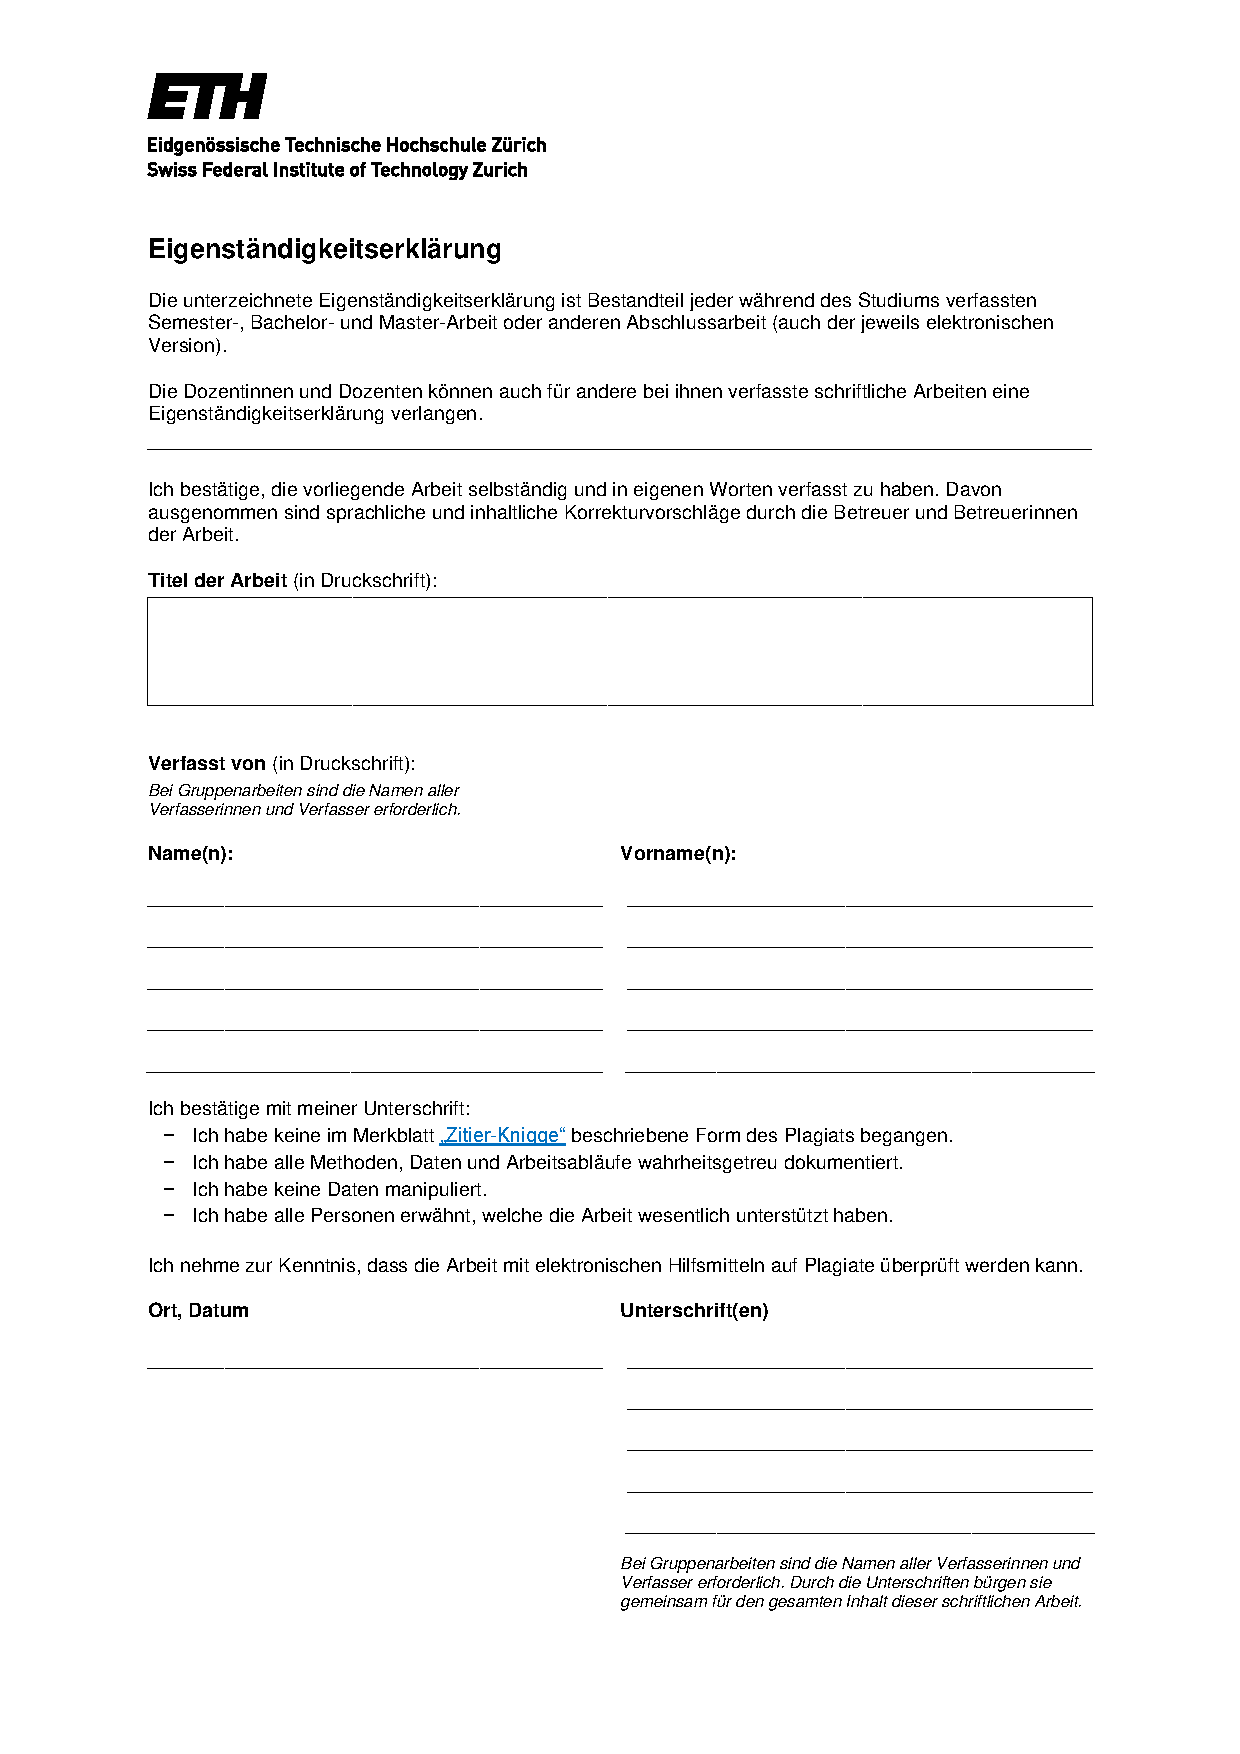
\includepdf[scale=0.8, pagecommand={}]
    {themen/pdfDateien/ethz_eigenstaendigkeitserklaerung.pdf}
\end{figure}

\end{verbatim}
